\documentclass[authoryearcitations]{UoYCSproject}
\usepackage[dvipdfm]{graphicx}
\usepackage[dvipdfm]{color}
\usepackage{amsmath, amsthm, amssymb}
\usepackage{a4wide}
\usepackage{simpsons}
\usepackage{subfig}
\usepackage{moreverb}
\usepackage{listings}
\lstset{language=Matlab,
label=DescriptiveLabel,
basicstyle=\small,
stringstyle=\ttfamily,
showstringspaces=false,
tabsize=2,
breaklines=true,
numbers=left
}

\author{Jose Manuel Calderon}
\title{Modeling Quantum Dots Using Geometric Primitives}
\date{2011-September-14}
\supervisor{Prof. Samuel L. Braunstein}
\MNC
\wordcount{1337}
\abstract{ \LaTeXe\ is a document markup and processing system built
  upon Donald Knuth's type-setting system, \TeX.}
   


\begin{document} 
\maketitle
\chapter{Introduction}

\chapter{Literature Review}
In this chapter we will look at and discuss some of the literature relevant to this project. 
In order to properly understand the system being modeled we will briefly touch on quantum mechanics
and some of the necessary mathematics. In the second section we will look at numerical methods with
particular focus on the finite difference method.
We will also look at various matrix representations that are present in the tools used for our
model. 
 
\section{Quantum Dots}
Since being discovered in the 1970's by Leo Esaki and 
Raphael Tsu quantum confinement in semiconductors has been of interest to physicists and engineers for numerous applications 
\cite{dots, reed}. Having at first demonstrated quantum confinement in one dimension, it was correctly predicted that 
confinement in two and three dimensions would be feasible \cite{dots}. A structure that exhibits 
quantum confinement in three dimensions is known as a quantum dots (QD from now on). Quantum wires and 
wells correspond to confinement in one and two dimensions respectively \cite{dots}. In this section we will discuss the
background necessary to be able to model QDs. This will include a brief look at some of the underlying physics with an 
explanation of the Schr\"{o}dinger Equation and 
presenting the properties of QDs themselves. 

\subsection{The Double Slit Experiment}
Before we dive into the Schr\"{o}dinger equation let us take a look at one of the most fundamental experiments in
quantum mechanics, the double slit experiment. While this section is not intended to cover all of the implications
of the double-slit experiment, it should give a basic understanding of the experiment and the reasons the experiment
helped shape our understanding of quantum mechanics. This experiment illuminates the fact that both matter and energy 
exhibit the properties of particles and waves \cite{qp}. 

\subsubsection{Background}
Before the beginning of the nineteenth century there had been an ongoing debate regarding the nature of light. While
several scientists, principally Leohnard Euler, advocated the theory that light behaved in a wave-like manner, the prevailing 
idea was Newton's corpuscular\footnote{A minute body or particle.} theory of light \cite{history}. While Newton himself admitted 
that viewing light as particles was not able to explain certain known properties of light; such as why two beams of light
can cross without the particles `hitting' each other off course. Still not satisfied, scientists searched for experiments that
would decide once and for all whether light behaved as a particle or as a wave \cite{history}. 

Between 1797 and 1799 Thomas Young performed experiments that supported the wave-like behavior of light. He accomplished this
by shining light through a screen with two pinholes onto a second screen. By observing the pattern of the light on the second 
screen he was able to deduce the wave-like behavior of light. In 1802 he published his observations in a paper titled \emph{On
the nature of light and colours} \cite{ralph}. On the observable pattern on the second screen he noted the following

\begin{quote}
The middle of the pattern is always light, and the bright stripes on each side are at such distances that the light coming to them from one of the apertures must have passed through a longer space than that which comes from the other by an interval which is equal to the breadth of one, two, three, or more of the supposed wavelengths, while the intervening dark spaces correspond to a difference of half a supposed wavelength, of one and a half, of two and a half, or more.
\end{quote}


In modern versions of the experiment, two parallel slits are used in place of the pinholes but most of the experimental setup 
is the same. We can now take a look at the experiment itself and further examine some of its implications. 

\subsubsection{Experimental Setup}
There are not many materials required for the most basic execution of this experiment. Only a point source of light, a
surface that can be used to detect light that shines upon it\footnote{This can come in many forms, it has been done with light
sensitive film, with digital sensors, and just plain surfaces that were then observed or photographed.} (we will call this the 
optical screen), and lastly a 
barrier with two small parallel slits that will sit between the light source and the optical screen. 

\paragraph{What we think should happen}
Let us take a moment to think about what would intuitively happen to the light passing through the two slits and reaching the
optical screen. First, if there was only one slit, we would expect that a band of light approximately the shape of the slit would 
appear on the optical screen. As this is indeed what occurs we would surmise that with two slits we would observe two bands of
light on the optical screen. As intuitive as that may seem, the actual result of the experiment produces a very different result.

\paragraph{What actually happens}
Interestingly, the pattern of light that is projected on to the optical screen is significantly different than the two 
bands of light we 
would expect to see. The observed pattern is what is known as an interference pattern. Figure \ref{fig:patterns}
shows the distribution of light on the optical screen for both the single and double-slit experiments.  

\begin{figure}
\centering
\subfloat[Single-slit pattern]{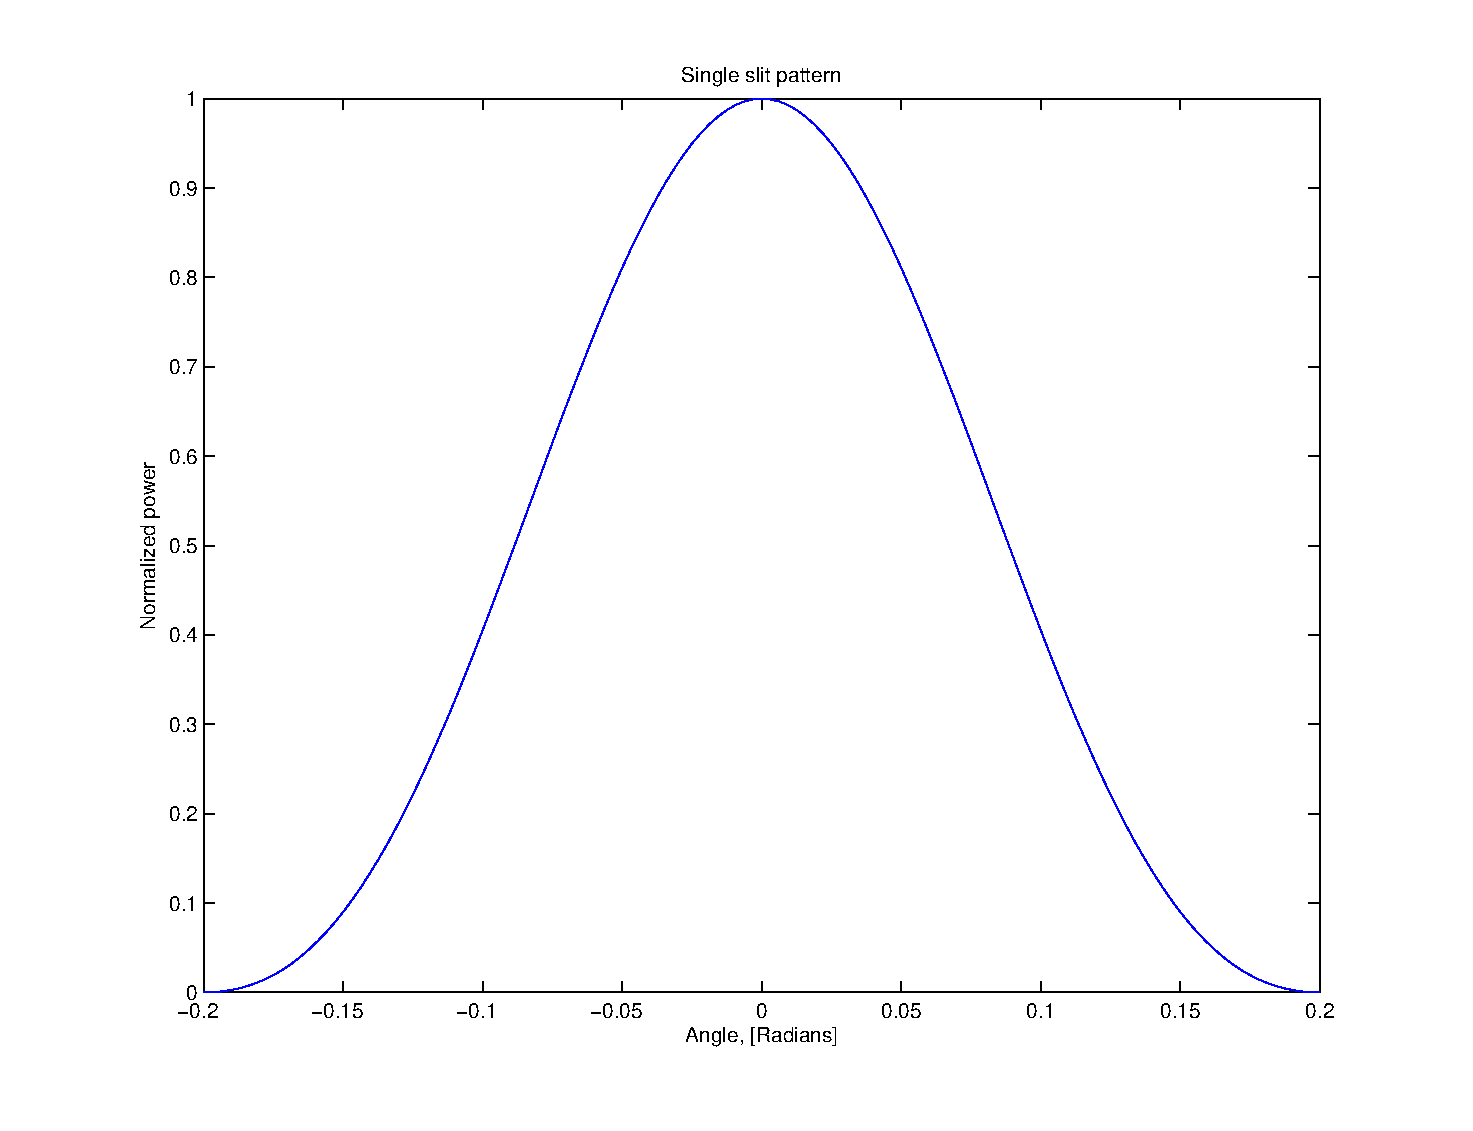
\includegraphics[scale=0.30]{figures/singleSlit.eps}}
\subfloat[Double-slit pattern]{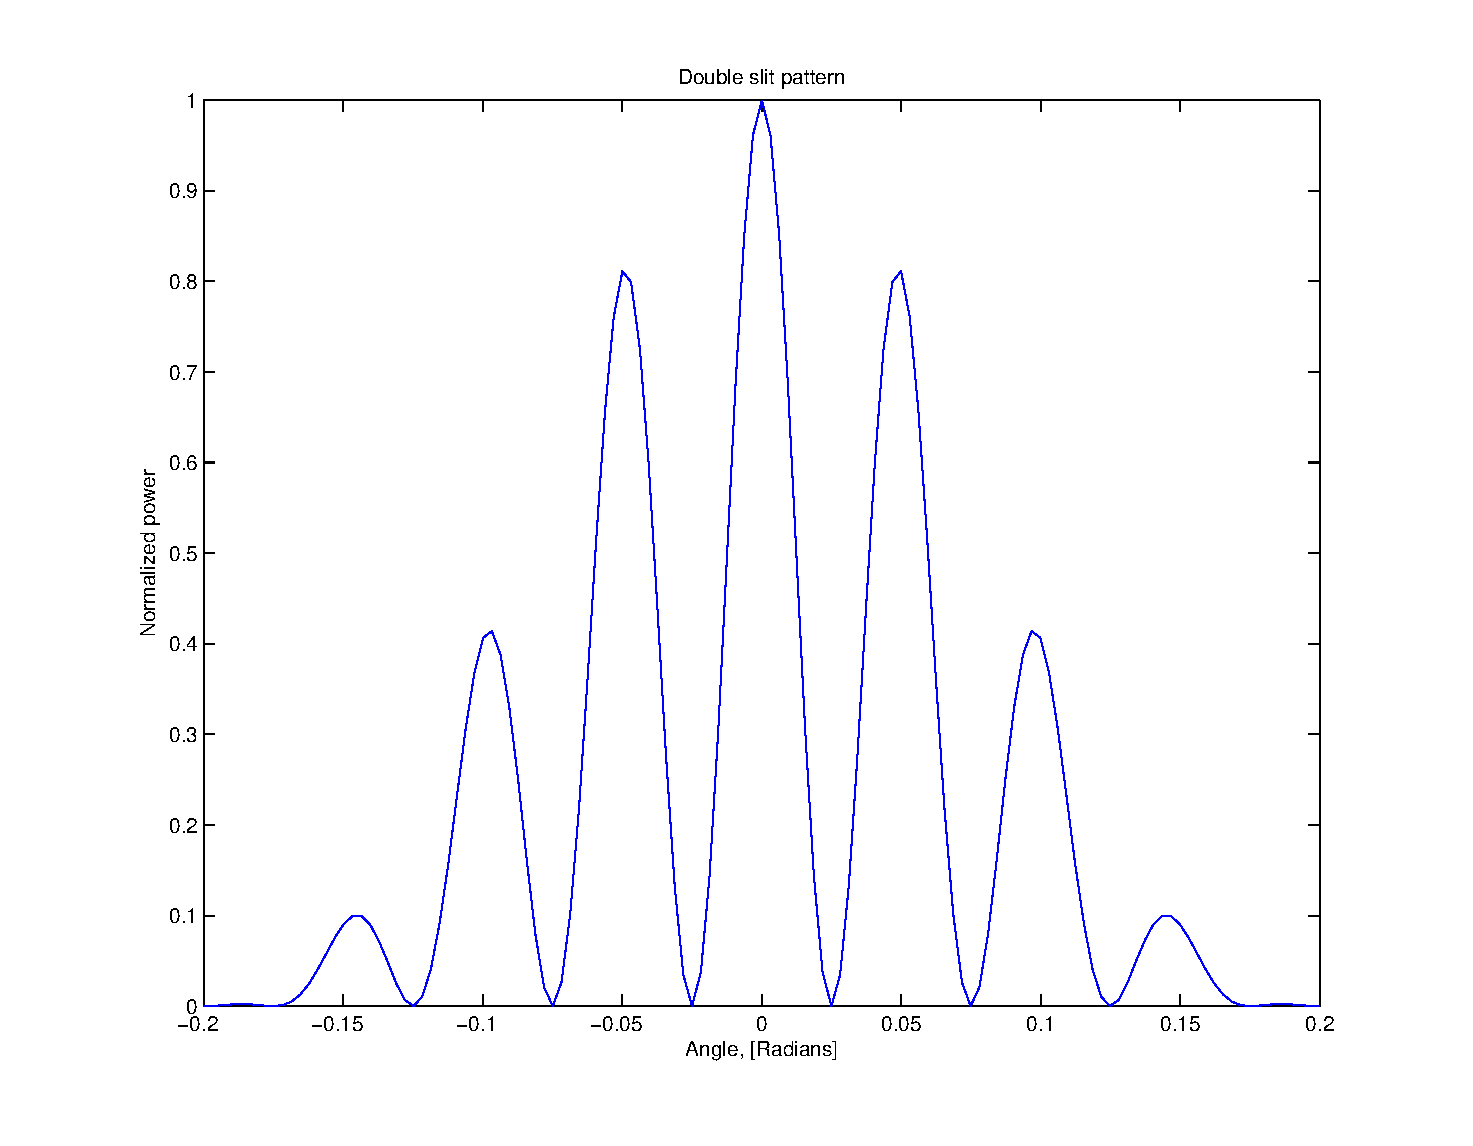
\includegraphics[scale=0.30]{figures/doubleSlit.eps}}
\caption{Single and double-slit patterns}
\label{fig:patterns}
\end{figure}


 \subsubsection{Consequences}
As this ran counter to the conventional wisdom of the time, it forced physicists to reevaluate the propagation
properties of light. The interference pattern lead physicists to draw similarities between the light and the propagation of 
waves. This ultimately resulted in the acceptance of light's particle/wave duality \cite{ralph}. Building on these findings
has lead to the modern understanding of quantum mechanics, and was the foundation that lead to the Schr\"{o}dinger equation, 
which is the equation we have used to model quantum dots. 

\subsection{The Schr\"{o}dinger Equation}
The Schr\"{o}dinger equation has been of the up most importance in physics since the beginning of the 20th Century. Solutions
to this equation can be used to describe systems ranging from the subatomic to the molecular and macroscopic. In this
section we will go over the foundation of the equation and produce the form to be used in our model. 

In classical mechanics we have the Hamiltonian operator that corresponds to the total
energy of a system. 

\begin{equation}
        H = K + V
\label{eq:totalEnergy}
\end{equation}

The total energy of a system is the sum of the kinetic energy ($K$) and the potential energy ($V$).
The kinetic energy is defined using the momentum, $p$, and the mass, $m$, of the object

\begin{equation}
        K = \frac{p^2}{2m}
\label{eq:K}
\end{equation}

In order to extend this to quantum systems we must adapt how we describe the momentum of a particle to
fit with the wave/particle duality \cite{qp}. This is accomplished using a few of the results from the early 
twentieth century. The Einstein's light quanta hypothesis and the de Brogile hypothesis \cite{qp, ricardo}. In 
1905 Einstein, building on the work of Max Planck,  
proposed the connection between the energy of a photon and its frequency $v$
\begin{equation}
E = hv = \hbar\omega
\label{einsteinHyp}
\end{equation}


Here $\hbar$ refers to the reduced Planck constant\footnote{Also referred to as the Dirac constant it is
the Planck constant divided by $2\pi$. The Planck constant reflects the proportion between the energy of a photon
and the wavelength of the respective photon. Expressed in joule seconds the reduced Planck constant is 
$1.054571726 \times 10^{-34} J \cdot s $ \cite{qp} } and $\omega = 2\pi v$, which is the same relationship
but using angular frequency. 

Almost twenty years later in 1924 de Brogile, again building on the work of Max Planck and of Einstein proposed
the following hypothesis

\begin{equation}
p = \frac{h}{\lambda} = \hbar k 
\label{brogileHyp}
\end{equation}

Which states that the momentum of a particle is proportional to the wavelength of that particle. Here $k$ refers to the 
wavenumber, or $k = \frac{2\pi}{\lambda}$. Wanting to create a wave equation, Schr\"{o}dinger decided to express the plane
wave, $\Psi$, in the trigonometric form and apply the hypotheses of Einstein and de Brogile \cite{ricardo}. 

\begin{equation}
\Psi (x, t) = e^{i(k\dot x-\omega t)}
\end{equation}

Using \ref{einsteinHyp} we are able to conclude that

\begin{equation}
E\Psi (x,t) = \hbar\omega
\label{einsteinPart}
\end{equation}

and because $\frac{\partial\Psi}{\partial t} = -i\omega\Psi (x,t)$

\begin{equation}
E\Psi (x,t) = i\hbar\frac{\partial}{\partial t}\Psi (x,t)
\label{einsteinPart2}
\end{equation}

We follow a similar process using the de Brogile hypothesis. Taking the second order partial derivative of
$\Psi$ with respect to $x$ 

$$\frac{\partial ^2}{\partial x^2}\Psi (x,t) = -k_{x}^{2}\Psi(x,t) $$

and remembering the postulate in \ref{brogileHyp} we get

\begin{equation}
p_{x}^{2}\Psi (x,t) = (\hbar k_{x})^2\Psi (x,t) = -\hbar ^2\frac{\partial ^2}{\partial x^2}\Psi (x,t)
\label{brogile2}
\end{equation}

This gives us the following substitution to use for our momentum,

\begin{equation}
p \rightarrow -i\hbar \nabla,\ p^2 \rightarrow -\hbar\nabla ^2
\label{eq:momentumSub}
\end{equation}

$\nabla$ here is the gradient operator in $n$-dimensions. Using this substitution and the result of 
\ref{einsteinPart2} we get the time-dependent Schr\"{o}dinger equation 


\begin{equation}
i\hbar\frac{\partial}{\partial t}\Psi (x,t) = -\frac{\hbar ^2}{2m}\nabla ^2 + V(x)
\label{eq:H}
\end{equation}

By assuming a trivial time dependence we can obtain the time-independent Schr\"{o}dinger equation. This replaces
the $i\hbar \frac{\partial}{\partial t}$ in \ref{eq:H} with $E$. With the wavefunction also having a trivial time
dependence we arrive at

\begin{equation}
E\psi = -\frac{\hbar ^2}{2m}\nabla ^2 + V(x) 
\label{eq:timeIndependent}
\end{equation}


Or

\begin{equation}
E\psi = \hat{H}\psi  
\label{eq:eigenSchrodinger}
\end{equation}

It is important to note at this point that the Schr\"{o}dinger equation does not have a mathematically rigorous 
derivation or proof. It is a heuristic derivation based on the hypotheses of Einstein and de Brogile and Schr\"{o}dinger's
desire to construct a wave equation that addresses the wave-particle duality \cite{ricardo, qp}. %CITE MORE HERE OMG OMG OMG PLEASE
%Seriously!!!
However, the equation and the reasoning behind it were very quickly validated when the Schr\"{o}dinger equation was used
to find an analytical solution to the hydrogen atom that correctly predicted the frequencies of the atom's spectral lines
\cite{qp}. This was done using Coulomb's law, which for the hydrogen atom states that the potential is symmetric in all dimensions
and only the distance from the nucleus is needed. Sch\"{o}dinger's equation has been used to find solutions to other atoms and
molecules, but usually analytical solutions are infeasible and the solutions are computed numerically. 


\subsubsection{Eigenvalue Problems}
The time-independent Schr\"{o}dinger equation can be treated as an eigenvalue problem for determining the energy levels
of a particle, which in our case is a quantum dot. An eigenvalue is a matrix equation of the form

\begin{equation}
Av = \lambda v
\label{eq:eigenDef}
\end{equation}

Here, $A$ is a square matrix and $v$ is a vector. The eigenvalue is the scalar $\lambda$ that by multiplying 
$\lambda$ with $v$ we arrive at the same result as multiplying $A$ with $v$ \cite{Hamming}. This is of interest
because when a vector $v$ that when multiplied by $A$ only changes in scale can have interesting properties in relation
to the system being analyzed. In our case, the Hamiltonian $\hat{H}$ is the differentiable operator associated with 
the energy of a quantum system. When discretized $\hat{H}$ forms a square matrix which is acting on the vector $\psi$
(which is the wavefunction). The time-independent Schr\"{o}dinger equation is therefore and eigenvalue equation where
$E$ is an eigenvalue acting on the same wavefunction. 
The real eigenvalue solutions to this equation are the energy levels
of the particle. These energy levels give us spectral information about the system being modeled. 


%\begin{equation}
%\nabla ^2 = \left(\frac{\partial ^2}{\partial x} + \frac{\partial ^2}{\partial y} + \frac{\partial ^2}{\partial z}\right) 
%\label{eq:laplace}
%\end{equation}



\subsection{Properties of Quantum Dots}
Quantum dots (QDs from this point on) are structures of semiconductors ranging between ??????
RANGE HERE ??????. Their size and properties make them ideal in modeling atomic physics in a
macroscopic system \cite{Li}. For this reason, they are sometimes referred to as artificial atoms 
??CITE RELEVANT HERE??.

\subsubsection{Potential Wells}

\begin{figure}[h]
  \centering
  \subfloat[Potential well]{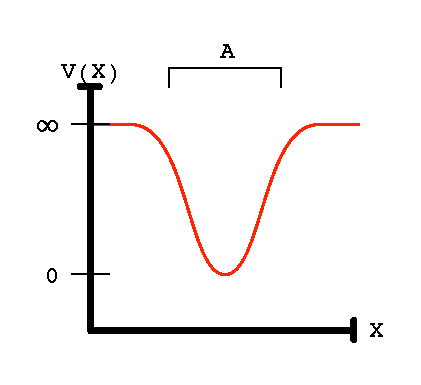
\includegraphics[scale=0.7]{figures/realWell2.eps}}
  \hspace{0.5 in}
  \subfloat[With approximate model]{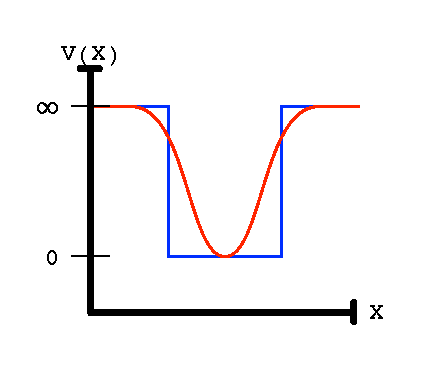
\includegraphics[scale=0.7]{figures/realWell.eps}}
    \caption{Difference between the assumed potential well and the more ``realistic'' well}
    \label{potWells}
\end{figure}

Quantum dots confine free carriers in all three dimensions. In order to understand the implications
of this we will look at how confinement is described by using \emph{potential wells}. A potential
well is an area of low potential energy, $A$, surrounded by areas of much higher potential, $B$. The difference 
in potentials is great enough that the wavefunction of a particle in $A$ would be zero anywhere in $B$\footnote{
remember that the wavefunction is a separate concept from the potential energy}, i.e.
the particle is \emph{confined} to area $A$. Figure \ref{potWells} illustrates an approximate ``shape'' of
an infinitely deep potential well in part (a) and how that corresponds to how physicist sometimes model
the same well when performing calculations \cite{dots, qp}. If area $A$ was defined in the $x$ dimension
then $V(x)$ would be

\begin{equation}
V(x) = \begin{cases}
          0 & \text{if $x$ is in $A$}  \\
          \infty    & \text{if $x$ is not in $A$} 
         \end{cases}
\label{vx}
\end{equation}


Using the model in part (b) of figure \ref{potWells} allows us to have a trivially identifiable well where confinement
takes place. This is the method with which physicists tackle analytical solutions to the Schr\"{o}dinger equation 
such as the ``particle in a box'' condition that we will investigate in a later section \cite{datta, qp, dots}.  
As mentioned earlier, when in a potential well the wavefunction of a particle cannot have enough energy to be present
outside of the well. This means that all possible wavefunctions are \emph{standing waves}\footnote{Standing
waves have a wavelength defined by $\frac{2l}{n}$ where $l$ is the length of the confinement and $n$ is a positive integer. 
Not all wavelengths can exist in an infinite well because the wavefunction must be zero at the boundaries.} in the confined area.


\begin{figure}[h]
 \centering
 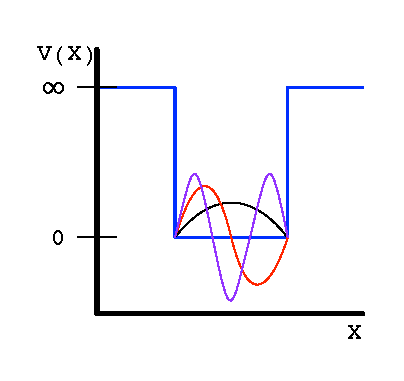
\includegraphics[scale=1]{figures/confined.eps}
 \caption{Standing waves in a infinite potential well}
\label{confined}
\end{figure}




When an electric field is present, the potential well changes in proportion to the direction and intensity of the
electric field. In figure \ref{fieldWell} we illustrate the effects of an electric field in the $x$ direction on 
the model potential well.

\begin{figure}[h]
  \centering
  \subfloat[With no electric field]{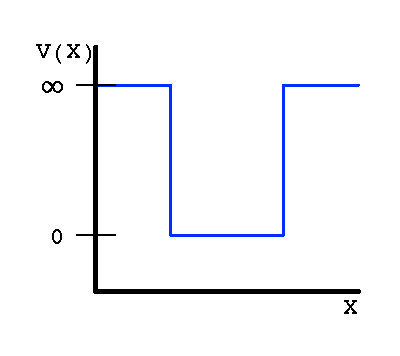
\includegraphics[scale=0.7]{figures/fakeWell.eps}}
  \hspace{0.5 in}
  \subfloat[With electric field]{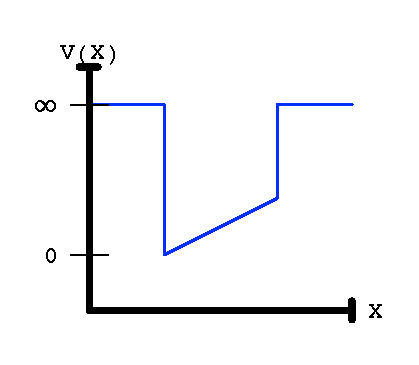
\includegraphics[scale=0.7]{figures/fakeFieldWell.eps}}
    \caption{How the potential well is affected by the presence of an electric field}
  \label{fieldWell}
\end{figure}

This means that when determining the potential energy for a point within $A$ we must also take into account the 
slope of the well created by the electric field. In the one 
dimensional case the potential energy is defined as a line with a slope that grows proportionally 
with the intensity of the electric field. This changes our equation \ref{vx} to

\begin{equation}
V(x) = \begin{cases}
          mx & \text{if $x$ is in $A$}  \\
          \infty    & \text{if $x$ is not in $A$} 
         \end{cases}
\label{vx2}
\end{equation}

Where $m$ is the slope of the line defining the electric field. We derived $m$ in our models by
taking the maximum value of the electric field and dividing it by the length of the dimension 
the electric field is acting on. By ensuring that the electric field was only acting on the $x$ dimension
we get

$$m = \frac{\text{Max(Electric Field)}}{L_x}$$

Where $L_{x}$ is the length of the $x$ dimension.

\subsubsection{Confinement in 3 Dimensions = Quantum Dots}
Now that we have an understanding of potential wells in one dimension we can easily expand this to higher
dimensionality. When a particle is confined in two dimensions, the system is known as a quantum wire. In three 
dimensions, we have a quantum dot. Whereas quantum wells and wires allowed a free carrier to potentially move in 
certain dimensions, a quantum dot restricts the free carrier to a finite three dimensional area \cite{dots}. 


\section{Finite Difference Method}
The finite difference method is one of several numerical methods that can be used in approximating
solutions to differential equations \cite{Hamming}. We will work through the use of the finite 
difference method and then discuss why this method was chosen over other possible alternatives. 

\subsection{Background}
The finite difference method arose due to the inherent inability of computing devices to perform
calculations using infinitesimal calculus \cite{Hamming, zhilin}. Because taking the space
between two points to its limit is impossible on a computer, estimates of the derivative must be
used. Additionally, as a continuous representation of a function is not feasible, a function is represented
by sampling values of the function at discrete points. The distance between these points will
be referred to throughout this section as $h$. 


\begin{figure}[h]
  \centering
  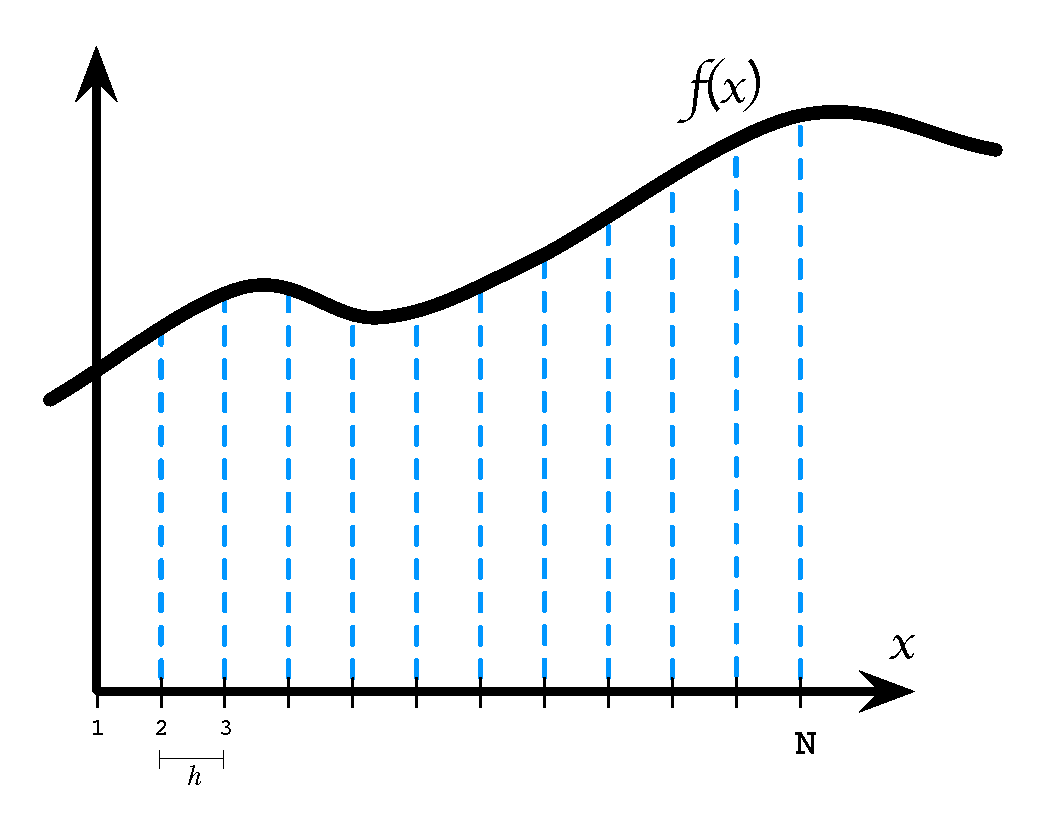
\includegraphics[scale=0.5]{figures/sampledFunc3.eps}
    \caption{Illustration of a function $f$ being sampled at discrete points}
\end{figure}

First we will define the difference operator used in FDM and then see how the difference 
operator along with the Taylor Series can be used to provide a numerical approximation of 
functions and their derivatives. 

\subsection{The Difference Operator}
A fundamental concept in the FDM is that of the difference operator. For any function 
$f$ this can be defined in three ways. As a \emph{forward difference}, a \emph{backward difference},
or as a \emph{central difference}. These are defined as follows

For the \emph{forward difference}:
\begin{equation}
\label{eq:forwardDiff}
\Delta f(x) \equiv  f(x + h) - f(x)
\end{equation}

For the \emph{backward difference}:
\begin{equation}
\label{eq:backDiff}
\nabla f(x) \equiv  f(x) - f(x - h)
\end{equation}

And for the \emph{central difference}:
\begin{equation}
\label{eq:centDiff}
\delta f(x) \equiv  f(x + \frac{1}{2}h) - f(x - \frac{1}{2}h)
\end{equation}


An important property of the difference operator that is utilized in our implementation is its linearity,
 and therefore
$$\Delta (af(x) + bg(x)) = a \Delta f(x) + b\Delta g(x) $$
where $a$ and $b$ are constants \cite{Hamming}. 

Just as with derivatives in the infinitesimal calculus, you can preform this operation repeatedly. Using the difference
operator twice, $\Delta [\Delta f(x) ] \equiv \Delta ^2 f(x) $, would correspond to the second derivative of the function. 
With the forward difference operator this is done as follows

\begin{align}
 \Delta ^2 f(x)&= \Delta [\Delta f(x)]  \nonumber\\
		&= \Delta [f(x + h) - f(x)] \nonumber\\
		&= \Delta f(x + h) - \Delta f(x) \nonumber\\  
		&= \Delta f(x + h) - (f(x + h) - f(x)) \nonumber \\
		&= f(x + 2h) - f(x + h) - (f(x + h) - f(x)) \nonumber \\ 
		&= f(x + 2h) - f(x + h) - f(x + h) + f(x) \nonumber \\
 \Delta ^2 f(x)	&= f(x + 2h) - 2f(x + h) + f(x) \label{eq:deltaSquared}
\end{align}

As we can see in equation \ref{eq:deltaSquared} the result for $\Delta ^2$ using the forward difference operator is based 
on the function's value at point $x$ and the succeeding two points $x+h$ and $x+2h$ respectively. Performing the same 
process using the central difference operator produces a slightly different approximation

\begin{align}
 \delta ^2 f(x)&= \delta [\delta f(x)]  \nonumber\\
		&= \delta [f(x + \frac{1}{2}h) - f(x - \frac{1}{2}h)] \nonumber\\
		&= \delta f(x + \frac{1}{2}h) - \delta f(x - \frac{1}{2}h) \nonumber\\  
		&= \delta f(x + \frac{1}{2}h) - (f(x) - f(x - h)) \nonumber \\
		&= f(x + h) - f(x) - (f(x + h) - f(x)) \nonumber \\ 
		&= f(x + h) - f(x) - f(x) + f(x - h) \nonumber \\
 \delta ^2 f(x)	&= f(x + h) - 2f(x) + f(x - h)\label{eq:delta2Squared}
\end{align}


Interestingly, we can see that equations \ref{eq:deltaSquared} and \ref{eq:delta2Squared} have similar coefficients,
with each point being shifted by $-h$. Following the same steps for the backward difference would result in each point
in equation \ref{eq:deltaSquared} being shifted by $-2h$. 

Now that we have defined the various difference operators 
we can now apply them to approximating the derivatives of a function. 

\subsubsection{Approximating Derivatives} 
Analytically, the derivative of a function at point $x$ is the limit

\begin{equation}
  f'(x) = \lim_{h\to0} \frac{f(x + h) - f(x)}{h} \nonumber
\end{equation}

We can see that this limit looks like our forward difference operator from equation \ref{eq:forwardDiff} multiplied
by $\frac{1}{h}$. Using this form and keeping $h$ at a predetermined discrete value (not taking the limit)
is a common way of approximating the derivative \cite{Hamming, wolfram, zhilin}. Replacing the numerator with
the backward difference or the central difference provides us with approximations using those difference operators. 
Backward difference

$$f'(x) = \frac{f(x) - f(x - h)}{h} $$

Central difference

$$f'(x) = \frac{f(x + \frac{1}{2}h) - f(x - \frac{1}{2}h)}{h} $$

More generally, to approximate a function's $n^{th}$ degree derivative you must calculate the $n^{th}$ degree
difference operator and then multiply by $h^n$ \cite{Hamming, weatherley4}. For a second order derivative using
the central difference operator we are left with

\begin{equation}
f''(x) = \frac{f(x + h) - 2f(x) + f(x - h)}{h^2}
\label{eq:2ndDegreeDiffOp}
\end{equation}

The choice of which difference operator to use depends largely on the problem at hand \cite{Hamming, weatherley}. 
Some problems with specific geometric requirements may benefit from the forward or backward difference schemes \cite{weatherley}.
Weatherly uses the example of modeling advection\footnote{Advection is the transport or movement of a substance or property
(like heat or salinity) in a fluid. Convection is a subset of advection, although some use them synonymously.} as a case
where one ``must be careful to use the approximation which utilises only values that are \emph{upwind} of the point where
we wish to compute the spatial derivative'' \cite{weatherley4}. Additionally, some temporal problems may only allow
either the forward or backward difference schemes. However, in cases where a point is equally influenced
from all directions, the central difference provides more accurate solutions \cite{Hamming, weatherley, weatherley4, analysis}.
In general cases such as these, the error for the forward and backward difference schemes is $O(h)$ whereas the error 
for the central difference is $O(h^2)$\footnote{Here, $h$ is very small, so $h^2$ is actually a smaller
error than $h$.} \cite{analysis, weatherley}. 
%The proofs for the error as found in \cite{weatherley} has been provided in the appendix. 

\subsection{Alternate Derivation using the Taylor Series}

Remembering the Taylor series expansion of a function

\begin{equation}
\label{eq:taylor}
f(x + h) = f(x) + f'(x)h+ \frac{f''(x)h^2}{2!} + \frac{f'''(x)h^3}{3!} + \dots + \frac{f^n(x)h^n}{n!} + R_{n}(x)
\end{equation}

Here $R_{n}(x)$ is the remainder term, which denotes the difference between the Taylor polynomial to the $n^{th}$ degree
and the actual function \cite{analysis}. 
We can `stop' the expansion at the desired derivative and solve for that derivative in order to attain an approximation. 
For example stopping at $f(x + h) = f(x) + f'(x)h$ and solving for $f'(x)$ presents us with

\begin{equation}
f'(x) = \frac{f(x + h) - f(x)}{h} - \frac{R_{1}(x)}{h}
\label{eq:taylorForward}
\end{equation}

Since our purpose is to approximate the derivative without having the actual analytic value our approximation looks like

\begin{equation}
f'(x) \approx \frac{f(x + h) - f(x)}{h}
\label{eq:taylorForwardApprox}
\end{equation}

This 1\textsuperscript{st} order approximation only uses one point to approximate the derivative. It is possible to use more 
points in the approximation by using the Taylor expansion for each desired point and then using a linear combination of these
polynomials \cite{farlow}. For example, if we required a 2\textsuperscript{nd} order approximation 
using the central difference between two point we could do this as follows

Using the Taylor expansions of two points $f(x+h)$
$$f(x+h) \approx f(x) + f'(x)h+ \frac{f''(x)h^2}{2!}$$ 

and $f(x-h)$
$$f(x-h) \approx f(x) - f'(x)h+ \frac{f''(x)h^2}{2!}$$ 

Summing these two together and solving for $f''(x)$ leaves us with

\begin{equation}
f''(x) \approx \frac{f(x + h) - 2f(x) + f(x - h)}{h^2}
\label{eq:2ndDegreeTaylor}
\end{equation}

As we can see the result is identical to the result in \ref{eq:2ndDegreeDiffOp}. Deriving the approximations through
the Taylor series allows a greater flexibility for customizing solutions to different problems as the approximation
can be derived from the specified points ($f(x+h)$ and $f(x-h)$ in our case). It allows extensions to greater accuracy when
more points are included in the derivation \cite{cambridge}.  

\subsection{Use with Schr\"{o}dinger Equation}
\label{sec:useWithSchro}
Remembering the time-independent Schr\"{o}dinger equation
\begin{equation}
E\psi = \hat{H}\psi = -\frac{\hbar ^2}{2m}\nabla ^2\psi + V\psi \nonumber
\end{equation}

As an eigenvalue problem our goal is to find the real eigenvalues in order to gain insight into the spectral information
of a quantum dot. 
For this example we will work in only one dimension and then in section \ref{sec:tensor} show how we can extend
it to three dimensions. 
In one dimension this requires finding approximations to $\frac{\partial ^2 \psi}{\partial x}$. We can set our
sample space on the $x$ axis to have a length of $1$ starting from the origin. The space between samples of the 
wave function is given by

$$\Delta = \frac{L}{N - 1} $$

Where $N$ is the number of samples we would like to use. If we choose to have $11$ samples this will give us
$\Delta = .1$. This will give us a vector of $11$ of $\psi$ wave function samples arranged as follows 

$$\begin{bmatrix} 
        \psi _0  \\
        \psi _{.1}  \\
        \psi _{.2} \\
        \vdots    \\
        \psi _{1} 
   \end{bmatrix}
$$


If we remember equations \ref{eq:2ndDegreeDiffOp} and \ref{eq:2ndDegreeTaylor} we can approximate the second 
derivative of $\psi$ at these points
using the function's value at that point and the adjacent points. So for $\psi _{n}$ this would give us
$$\frac{d ^2 \psi _{n}}{dx} = \frac{\psi _{n-\Delta} - 2\psi _{n} + \psi _{n+\Delta}}{\Delta ^2} $$

%where $h \equiv \Delta$. 
Each point in our sample space has an equivalent equation. We can of course create the following matrix representation

\begin{equation}
\frac{1}{\Delta ^2}\begin{bmatrix}
                -2     &   1    &     0    &     0   & \cdots & 0 \\
                1      &  -2    &     1    &     0   & \cdots & 0 \\
                0      &   1    &    -2    &     1   & \cdots & 0 \\
                \vdots & \vdots &   \vdots & \vdots  & \ddots & \vdots \\
                0      & \cdots &    \cdots     &     0   &    1   & -2
              \end{bmatrix}\cdot \begin{bmatrix} 
                                        \psi _1  \\
                                        \psi _{2}  \\
                                        \psi _{3} \\
                                        \vdots    \\
                                        \psi _{N} 
                                   \end{bmatrix}
\label{eq:kinetic}
\end{equation}

The dimensions of the matrix correspond to the number of samples, so for N samples the resulting matrix will be
$N \times N$ in size. This matrix represents the kinetic energy portion of the Schr\"{o}dinger equation. Without
any potential the kinetic energy matrix is equivalent to the Hamiltonian operator and we now have enough information
to solve the eigenvalue problem $E\psi = \hat{H}\psi$. In order to calculate the energy of the system taking into 
account the potential $V$ we construct a diagonal $N \times N$ matrix where the values are the potential energy at each sample
point. Therefore, $V_{nn}$ will equal the potential at point $x_{n}$\footnote{More information on the construction of
the potential energy matrix is discussed in section \ref{sec:potential}}. This will take the following form

\begin{equation}
\begin{bmatrix}
                V(x_1) &   0     &   \cdots & \cdots &     0 \\
                0      &  V(x_2) &    0     &        &  \vdots \\
                \vdots &   0     &   \ddots &        &  \vdots \\
                \vdots &         &          & \ddots &     0 \\
                0      & \cdots  &   \cdots &   0    &   V(x_N)
              \end{bmatrix}
\label{eq:potential}
\end{equation}

This matrix is added to the kinetic energy matrix with gives us our new Hamiltonian operator. At his point
we have sufficient information to numerically solve for the eigenvalues of this system, giving us the spectral information
of the quantum dot.  
 

Now that we have looked that the principles of the FDM, we can now look at how to apply it to the Schro\"{o}dinger equation.

\subsection{Sources of Error}

\section{Representation of Shapes}
In reaching our goal of modeling quantum dots of various shapes, we must look into how shapes can be defined and used in 
calculations. There are several methods and techniques in the representation of three dimensional shapes on a computer. 
Computer graphics deals with the representation of shapes to a great degree, with many sophisticated techniques having been 
developed for 3D-modeling, computer aided design (CAD), and computer gaming to name a few. Our purposes may not require
many of the sophisticated techniques that others have developed as we only require sufficient information to determine if
a point is inside or outside of a given shape. 

In the first subsection we will look at some of the prevailing techniques for representing shapes on a computer. Then we will 
look at our chosen method in greater depth. 

\subsection{Possible Representations}
Researchers have developed many methods for representing shapes in computation. Generally a distinction is made between what is 
known as \emph{raster graphics} and \emph{vector graphics} \cite{bors}; for ease of understanding we will look at these two 
paradigms in two dimensions and then explain how they can expand to three. 

\subsubsection{Raster Graphics}
Raster graphics are relatively simple to understand, but can become quite complicated for certain purposes. At its most basic, 
a two dimensional raster graphic is simply a grid made up of discrete cells (also called pixels) that are individually colored.  
Each cell withing the grid has an associated value. Depending on the coloring scheme in place the value determines the 
color of the associated cell. 

\begin{figure}[h]
  \centering
  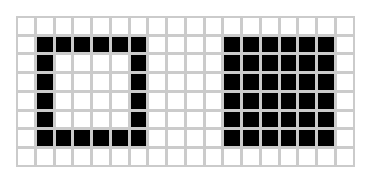
\includegraphics[scale=1.0]{figures/rasterSquare.eps}
    \caption{Raster graphic depicting an empty and a filled square}
  \label{rasterSquare}
\end{figure}

In the case of figure \ref{rasterSquare} each cell is defined by a single bit where \verb+1+ colors the cell black and
\verb+0+ colors the cell white\footnote{In many cases, such as in a monochromatic LCD screens, it would simply be 
`on' and 'off' for each pixel}. This allows the description of an image to be stored as a matrix of values in memory. 
The matrix for the image in \ref{rasterSquare} would look as follows

\begin{verbatim}
                0 0 0 0 0 0 0 0 0 0 0 0 0 0 0 0 0 0
                0 1 1 1 1 1 1 0 0 0 0 1 1 1 1 1 1 0
                0 1 0 0 0 0 1 0 0 0 0 1 1 1 1 1 1 0
                0 1 0 0 0 0 1 0 0 0 0 1 1 1 1 1 1 0
                0 1 0 0 0 0 1 0 0 0 0 1 1 1 1 1 1 0
                0 1 0 0 0 0 1 0 0 0 0 1 1 1 1 1 1 0
                0 1 1 1 1 1 1 0 0 0 0 1 1 1 1 1 1 0
                0 0 0 0 0 0 0 0 0 0 0 0 0 0 0 0 0 0
\end{verbatim}

Not surprisingly, this method is commonly referred to as a \emph{bitmap}, although this has also become a way to 
reference any raster image that has not undergone any form of compression. 
For monochromatic images this system is extremely straight-forward. Displaying the image is a matter of iterating through
the representation in memory and setting the pixels accordingly. For color images we would not be able to use bit values for
each cell and instead would need to store the appropriate convention for that particular format. A common convention is to store
eight bits for each color component; Red, Green, and Blue (RGB)\footnote{More modern representations also include and `Alpha'
component for the level of transparency.}. This gives over 16 million different possible colors. In some image processing
toolkits such as \verb+MATLAB+ store each component in a separate matrix so as to facilitate processing the individual components
separately. 

For our purposes a simple bitmap would be sufficient to represent the
\emph{in} or \emph{out} information we require for each QD. Representing a QD would be a matter of 
storing a three dimensional matrix (for the spacial dimensions) and setting the bits that are within
the Quantum Dot to \verb+1+ and leaving all the other bits at \verb+0+. This trivializes the process of 
determining when a sample point is withing the quantum dot or not as it is encoded into the definition of 
each shape. However, there are two main
issues that make raster images less suitable for our purposes. Raster images are resolution dependent. This means that
each image is specific at a specific resolution and that scaling the image to different resolutions is not possible in a 
straightforward way, usually (read almost always) resulting in loss of quality in the resolution. For example, let us
create a representation of a circle in a $10x10$ grid

\begin{figure}[h]
  \centering
  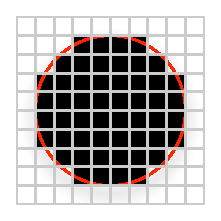
\includegraphics[scale=1.0]{figures/rasterCircle.eps}
    \caption{Circle in raster representation, with a red outline of the ``true'' circle}
  \label{rasterCircle}
\end{figure}

In \ref{rasterCircle} we have superimposed a red circle on the image to better illustrate the actual dimensions of the circle. 
Without the mathematical representation of the circle (what is in red), we would not know how to scale this image if instead of
$10x10$ we chose to use a $20x20$ grid. This is because the ``true'' shape of the circle is lost in the raster representation.  

\subsection{Geometric Primitives (Vector Graphics)}

This is where geometric primitives are useful. A geometric primitive is a `basic' building block for more complex shapes. 
Much in the same way that substances are made up of a finite number of elements, complex shapes can be constructed using
a finite set of primitives. 

An example set of primitives for two dimensions would be

\begin{itemize}
        \item lines
        \item points
        \item triangles
        \item circles
\end{itemize}

The list of primitives may seem short, but by combining these primitives in various ways we are able to define more
complex shapes. For example, two $90^{\circ}$ isosceles triangles can be placed together at their hypotenuse to form 
a square. In fact, triangles can be used to form any polygon. 

\chapter{Design and Implementation}
Now that we've looked at the necessary background information we can construct a program that will 
compute our numerical approximations. First we will look at how to represent our geometric primitives 
and how to construct the potential energy matrix from a set of shapes. We can then easily construct
the matrix for the kinetic energy. After we have looked at the basic construction of the program, we 
will look at using sparse matrix representations in order to keep the memory usage as small as possible.

\section{Sparse Matrix Representations}
The implementation that is described in this chapter uses \emph{sparse matrix} representations of the
kinetic and potential energy matrices. In this section we will explain how sparse matrices work and the advantages
they allow for certain problems such as our own. 

A sparse matrix is one in which most of its values will be zero. Because the non-zero values are arrange `sparsely'
storing all the elements of the matrix is seen as wasteful. 

\begin{figure}
\centering
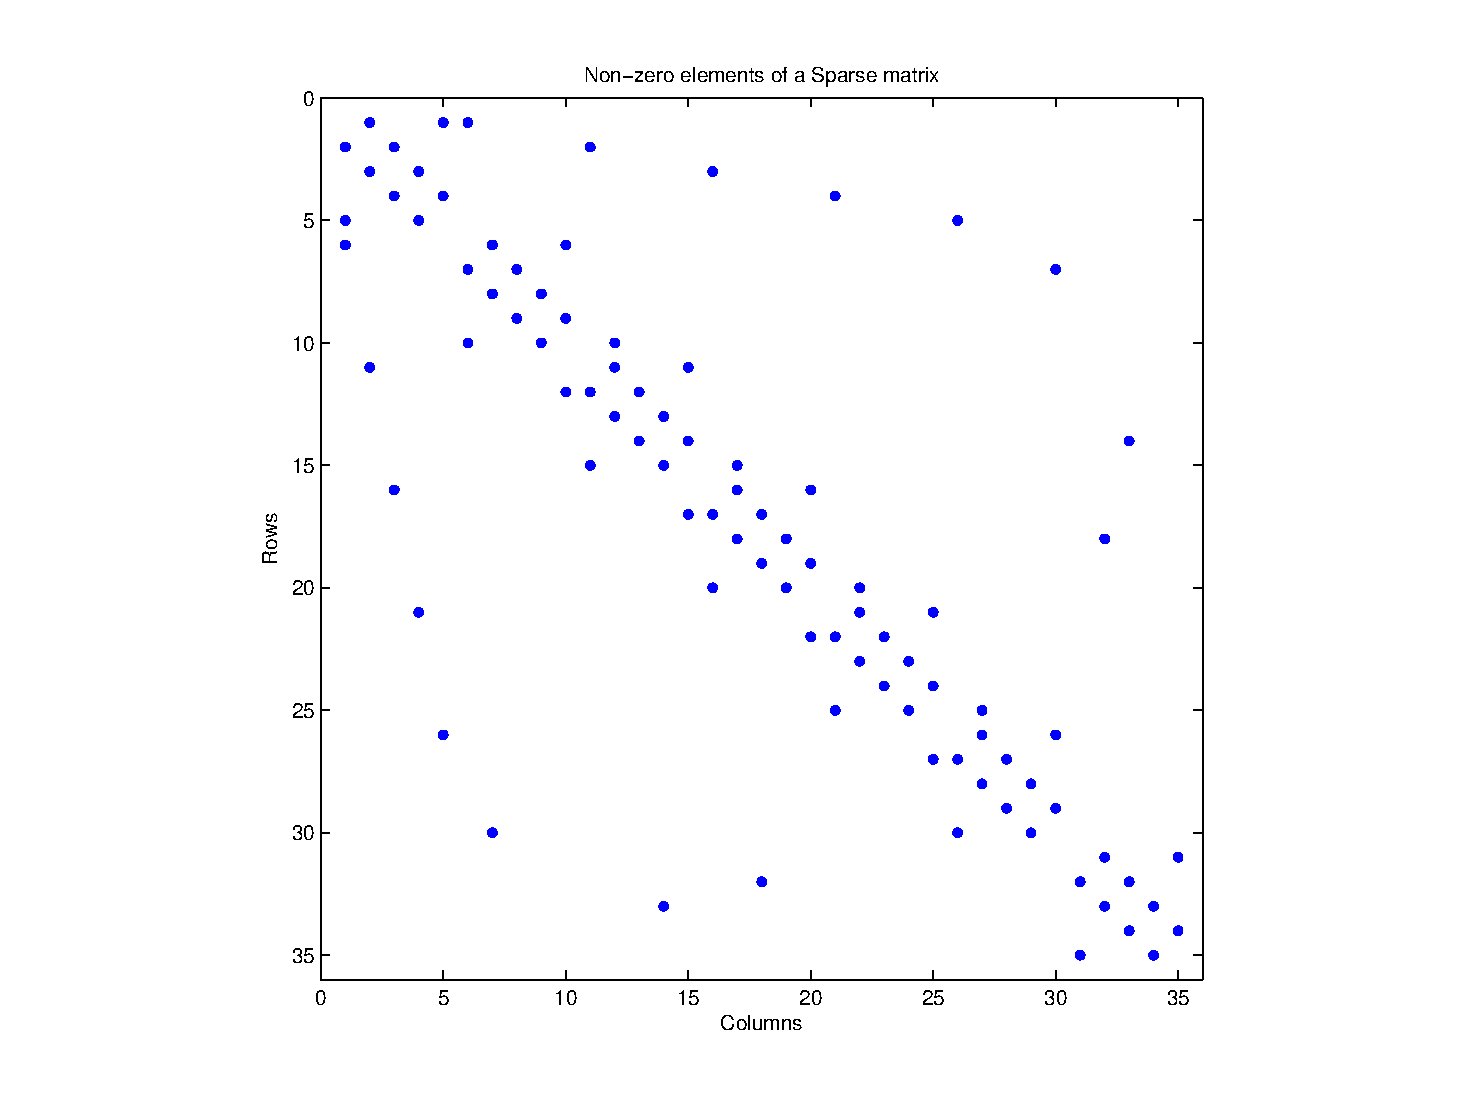
\includegraphics[scale=0.5]{figures/sparseVisual.eps}
\caption{The colored dots are the non-zero elements of the sparse matrix}
\label{sparseExample}
\end{figure}

Figure \ref{sparseExample} displays a $[35 \times 35]$ matrix where most of the elements are zero. Using memory
to store the empty parts of the matrix is unnecessary, it would be much more efficient to store only the location 
and value of the non-zero elements. This is exactly what sparse matrix representation accomplishes. 

At its core, the sparse matrix representation of a matrix is stored as 3 vectors. Two vectors store the 
indices of the non-zero elements, while the third vector stores the value of those elements. 

\begin{equation}
\begin{array}{c c c}
X\text{ Index} & Y\text{ Index} & \text{Value} \\
\begin{bmatrix} 
                1 \\
                2 \\
                2 \\
                3 \\ \end{bmatrix} & \begin{bmatrix}          
                                           1 \\
                                           1 \\
                                           2 \\
                                           3 \\ \end{bmatrix} & \begin{bmatrix}
                                                                        5 \\
                                                                        -1 \\
                                                                         4 \\
                                                                          6 \\
                                                                \end{bmatrix}
\end{array}
\label{eq:sparse}
\end{equation}

The three vectors in \ref{eq:sparse} define the following matrix

\begin{equation}
\begin{bmatrix}
5   & 0  & 0 \\ 
-1  & 4  & 0 \\
 0  & 0  & 6 \\
\end{bmatrix}
\end{equation}

In \verb+MATLAB+ we can define sparse matrices using the \verb+sparse+ function. The parameters passed to the function
are the three vectors that define the matrix. 
In order to define a sparse matrix that has elements only along the diagonal (much like we will do with the potential
energy matrix), the vectors that define the indices will both be an $n$ element long vector from $1$ to $n$ where $[n \times n]$
is the size of the matrix. Therefore executing \verb+sparse(1:n,1:n,1)+ in \verb+MATLAB+ will create an $[n \times n]$ sparse
identity matrix. It is also possible to pass an entire matrix to the \verb+sparse+ function. This will return an new sparse
matrix version of the passed matrix. 

\subsubsection{Advantages for our implementation}
The size of the potential and kinetic energy matrices correspond to the number of sample points in the system. 
Because we will be using a sample cube (where the number of samples is the same in all dimensions) this means
that is we desire a sample size of $n$ per dimension, we have $n^3$ total sample points in the system. The 
matrices that represent the system will always have one column and one row for each sample point. This gives
us $n^D \times n^D$ sized matrices, where $D$ is equal to the number of dimensions. 

If the simulation was a one dimensional problem
using the sparse representation would not be as crucial. Even using $n = 500$ nets us a kinetic energy matrix of
$500 \times 500$ which is very manageable in memory. It is because we are modeling a three dimensional system that
necessitates the use of sparse matrices for both the kinetic and potential energy matrices which will both be
$n^3 \times n^3$, so even smaller sample rates such as $n = 50$ produces matrices on the order of $125000 \times 125000$.




\section{Potential Energy Matrix}
\label{sec:potential}
In this section we will focusing on the implementation of the setup of the potential energy matrix
from the Sch\"{o}dinger equation, or $V$ from $E\psi = -\frac{\hbar ^2}{2m}\nabla ^2\psi + V\psi $.

The potential energy depends on the shape of the quantum dot, and the electric field present (if any). 
%We should reference back to the diag



Each point the sample cube must be iterated through in order to determine whether it is within the QD. 
Because the diagonal of the potential matrix is indexed by a single integer we must translate the 
coordinates of a point into a unique integer value 
that corresponds to location of each point. Additionally, we do not care about the spacing or the absolute location
of the points in
the sample cube, only their relative location. Therefore we count the points using a specific pattern, counting
the samples along the x-axis until we have reached the full length. Then we increase the y-axis value and
begin counting along the x-axis once again. Figure \ref{indexNum} illustrates a two dimensional example. 
In order to add a third dimension it helps to think of three dimensions as a ``stack'' of  two dimensional grids,
ensuring that you continue the index count from the end of the last grid.

\begin{figure}[h!]
  \centering
  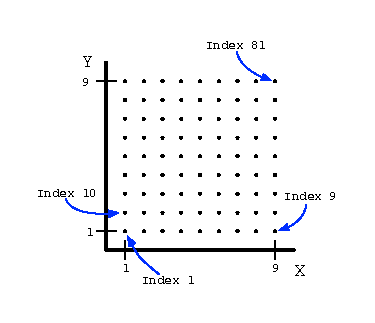
\includegraphics[scale=1.5]{figures/indexNumbering.eps}
  \caption{Two dimensional example of numbering scheme}
\label{indexNum}
\end{figure}

For a three dimensional sample space coordinate $(1,1,1)$ must translate to the first index, 
$(2,1,1)$ the second and so on. If the grid in figure \ref{indexNum} was only the first layer in a three dimensional 
space after having counted $(9,9,1)$ which is assigned index 81, you iterate to $(1,1,2)$ which would be assigned index 82.
The following function was written to take an arbitrary coordinate and return the appropriate index.
 
\begin{lstlisting}[caption={Index value from sample point},
label=lst:coordToIndex]
function index = coordToIndex3D(x, y, z, n)
    index = ((z-1)*n^2) + ((y-1)*n) + x;
end
\end{lstlisting}

By iterating through all the points in the sample cube using \verb+for+ loops we can determine the appropriate index
for each sample. While we require a running count to determine the index of the point in the matrix, 
we need the absolute position of each
point in order to determine whether the point is within the QD. This can be calculated from the iterated count
using the following

\begin{lstlisting}[caption={Finding the absolute coordinates}, label=absoluteCoord, firstnumber=16]
xVal = (x-1) * delta;
yVal = (y-1) * delta;
zVal = (z-1) * delta;
\end{lstlisting}

By iterating through the number of samples in each dimension we now have both the appropriate index value for the 
potential energy matrix, and we have the absolute position of each point. Once we determine whether the sample point
is within the QD we can assign the appropriate potential value to the correct index in $V$. 

\subsection{Determining if a point is within a primitive}
The shape of the quantum dot is made up of a set of primitives. We use a \verb+MATLAB+ cell array in order to store
the set of primitives. For our purposes a cell array is simply an array of matrices where each matrix is the
definition of a primitive. We pass the cell array and the current coordinates (absolute position) into a function
that returns a boolean. Either the point is within the set of primitives or it is not. Each primitive is defined
by a one dimensional matrix (can also be referred to as a vector). However, as the different primitives are described
differently, they have different
formats. In order to differentiate the primitives from each other each definition begins with an
integer value of 1, 2, or 3. 1 corresponds to spheres, 2 corresponds to rectangular prisms, and 3 corresponds to 
cylinders. This makes it easy for the program to determine which primitive it is currently working on and gives us the
following format. 

$$\begin{array}{r l}
        Spheres &= [1, OriginX, OriginY, OriginZ, Radius] \\
        Rectangular Prisms &= [2, OriginX, OriginY, OriginZ, Length, Width, Depth] \\
        Cylinders &= [3, Point1X, Point1Y, Point1Z, Point2X, Point2Y, Point2Z, Radius] 
  \end{array}$$

\subsubsection{Points within a sphere}
We will begin by describing how to determine whether a point is inside of a sphere. Because of their complete
symmetry a sphere is the simplest to test out of our primitives. A sphere is defined by its origin ($(x,y,z)$)
and its radius. A given point is within the sphere if the euclidean distance from that point to the origin of
the sphere is less than or equal to the radius of the sphere. The \verb+MATLAB+ code for this is very simple.

\begin{lstlisting}[caption={Determining if a given point is in a given sphere}, label=lst:sphere]
function isIn = isInSphere(x,y,z, sphr)
	
        dst = sqrt((x-sphr(1))^2 + (y-sphr(2))^2 + (z-sphr(3))^2);
        if (dst <= sphr(4))
                isIn = 1;
        else
                isIn = 0;
        end
end
\end{lstlisting}

\subsubsection{Points within a cylinder}
The manner in which we define cylinders is quite simple, two points are used to define the center line of the
cylinder and a radius is used to define the area around the center line. If a point is within the two ends of the
cylinder all we need to check is the distance from the center line and compare that to the radius. Conversely, if the
point is outside of the two end points it is not in the cylinder. In order to accomplish this we use the parametric
equations of the center line. 

\paragraph{Parametric Equations of a Line}
Given two points, $P1(x,y,z)$ and $P2(x,y,z)$, the parametric equations for the line that passes through the two points
is defined as

\begin{equation}
\begin{array}{r l}
x(t) &= P1(x) + t * (P2(x) - P1(x)) \\
y(t) &= P1(y) + t * (P2(y) - P1(y)) \\
z(t) &= P1(z) + t * (P2(z) - P1(z)) 
\label{eq:paramet}
\end{array}
\end{equation}

This gives us a single parameter, $t$, that describes any point on the line. If $t = 0$ you can see that the
point is $P1$, and if $t = 1$ the point is then $P2$, this means that any point on the center line within the cylinder
will satisfy 

\begin{equation}
0 \leq t \leq 1 
\label{eq:tBoundary}
\end{equation}

Given a third point $P3$ we can use dot products to 
project $P3$ onto the line and get the minimum value for $t$, which corresponds to the point on the line 
that is closest to $P3$. 

\begin{equation}
t = \frac{P3 \cdot (P2 - P1) - P1 \cdot (P2 - P1)}{(P2 - P1) \cdot (P2 - P1)}
\label{eq:dotProd}
\end{equation}

Here $A \cdot B$ is the dot product of $A$ and $B$. 

Once we have $t$ we can do our first check. Remembering that $t$ must satisfy the constraint in \ref{eq:tBoundary} 
to have any possibility
of being within the cylinder, we can forgo any further work if the constraint is not satisfied. If $t$ does fall within the
boundaries of the center line we must compute the distance from the projected point to $P3$. The projected point is
found by entering our $t$ value into the parametric equation \ref{eq:paramet} and then calculating the euclidean
distance between the two points. If the distance is within the defined radius then the point is within the cylinder. 

This was all accomplished using the following function. 


\begin{lstlisting}[caption={Finding if a point is within a cylinder}, label=lst:isInCyl]
function isIn = isInCylinder(x,y,z, cyl)
	
        cylRange = cyl(4:6) - cyl(1:3);
        t_min = ( (dot([x,y,z], cylRange) - dot(cyl(1:3), cylRange))... 
                        / dot(cylRange, cylRange));
        
        if (t_min < 0 || t_min > 1)
                isIn = 0;
                return;
        end
        
        pointOnLine = parametricPoint(cyl, t_min);
        difference = [x,y,z] - pointOnLine;
        distFromLine = sqrt( dot(difference, difference));
        
        if (distFromLine > cyl(7))
                isIn = 0;
        else
                isIn = 1;
        end

        function p = parametricPoint(cyl, t)
                p = zeros(size(cyl(1:3)));
                
                cylRange = cyl(4:6) - cyl(1:3);
                p(1) = cyl(1) + t * cylRange(1);
                p(2) = cyl(2) + t * cylRange(2);
                p(3) = cyl(3) + t * cylRange(3);
        end		
end
\end{lstlisting}

Because only cylinders required the $t$ value to be translated into the actual point the function 
\verb+parametricPoint(cyl, t)+ was written as a private function within the body of \ref{lst:isInCyl}.

\subsubsection{Points in a Rectangular Prism}
We can apply many of the same principles we used in testing points in a cylinder to points in a rectangular prism.
Having a corner point (defined as the origin) and the length of each dimension we have enough information to make a
parametric equation for the three lines that intersect the origin. The main difference between using parametric 
equations for the rectangular prism and the cylinder is that we only need to test that $t$ is within the constraints 
in \ref{eq:tBoundary} for each dimension. We can illustrate this easily using a two-dimensional example

\begin{figure}[h!]
  \centering
  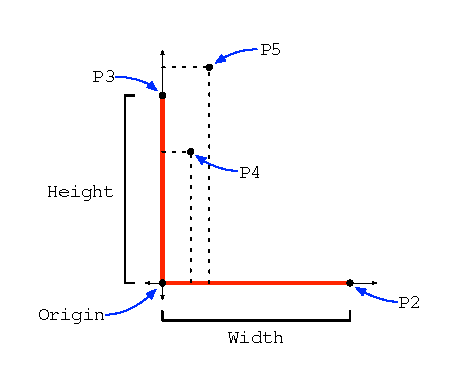
\includegraphics[scale=1.2]{figures/recPrism.eps}
  \caption{Points projected onto the sides that intersect the origin}
\label{recPrism}
\end{figure}

Because we need two points for each line segment to be defined by a set of parametric equations we must add the
width, height, and depth to the origin to get the necessary three points. Each new point defines a line segment 
that intersects with the origin. We then project the test point onto each of these lines. As with cylinders,
if any of these projections lie outside of the line segment then the point cannot possibly be within the prism. 
The test point must have a $t$ value that satisfies the constraint in \ref{eq:tBoundary} for \emph{each} line segment
to be within the prism. In the two-dimensional example shown in figure \ref{recPrism}, $P4$ satisfies the constraint
for both line segments while $P5$ does not. Therefore, as is visually apparent, $P4$ lies within the square whilst 
$P5$ does not. Because of the similarities to the function defined in \ref{lst:isInCyl} we will only list the
important differences for our \verb+isInRecPrism+ function. At the beginning of the function we define the three needed
points using the width, height, and depth found in the definition of the prism. 

\begin{lstlisting}[caption={Implementation of finding points that lie within a rectangular prism}, label=lst:isInPrism]
function isIn = isInRecPrism(x,y,z, recPrism)
    
        point2 = recPrism(1:3) + [recPrism(4), 0,0];
        point3 = recPrism(1:3) + [0,recPrism(5), 0];
        point5 = recPrism(1:3) + [0, 0, recPrism(6)];
\end{lstlisting}

We then calculate the $t$ value for each test point onto each of the three lines. This is done using dot products
in the same manner it was done in \ref{lst:isInCyl}. This gives us three $t$ values, which we have named
\verb+t_minX, t_minY,+ and \verb+t_minZ+. Using these values we can write a boolean expression to determine
whether the point is inside the prism. As with all boolean expressions there are multiple equivalent ways
of expressing them. In this case we chose to test for the point being \emph{outside} of the prism. Therefore
we have a set of \verb+OR+ expressions. Because \verb+MATLAB+ short-circuits\footnote{Short circuiting a boolean 
expression means that the runtime system will not evaluate the rest of the boolean expression once it has enough
information to know the outcome of the overall expression. For \texttt{OR} gates, this means that if any of the
statements is true none of the other statements need to be evaluated. For \texttt{AND} gates, if any are false
than the entire expression is false.} boolean expressions is any of the \verb+t_min+ values are outside of the
constraints the function indicates that the point is not within the prism and returns. 

\begin{lstlisting}[caption={Boolean expression for points in a RecPrism}, label=lst:boolExpr, firstnumber=19]
  if ((t_minX <= 0 || t_minX >= 1) || (t_minY <= 0 || t_minY >= 1) || ...
          (t_minZ <= 0 || t_minZ >= 1) )
       isIn = 0;
       return;
  else
       isIn = 1;
  end
\end{lstlisting} 

\subsubsection{Putting them all together}

Now that we have functions to determine whether a point is in a given primitive, we are able to write the ``glue''
code that allows us to take any set of primitives that make up a shape and determine if a point is within
the shape. By finding the length of the cell array that stores the primitives we can iterate over each primitive
checking the leading value of each primitive's vector and calling the appropriate function. 

We now have all of the information we require to construct the potential energy matrix. For each point we have
the correct index and we can determine whether that point is inside the QD. If a point is within the QD we 
want to store the value of the electric field at that point, otherwise we want to store our maximum potential. 
Using the sparse matrix representation, we create a vector of length $N^3$ where $N$ is the number of samples per
dimension, and
store the appropriate value for each sample point in its corresponding index. Once all of the values have been set
for this vector, we use the \verb+spars(coordinate1, coordinate2, vector)+ function to create our $N^3 \times N^3$
sparse matrix.

The final product of these steps is the \verb+calcVPotential.m+ matlab function that can be found in the appendix. 

\section{Kinetic Energy Matrix}
As compared to the potential energy matrix, the construction of the kinetic energy matrix is quite simple. 
If we remember from section \ref{sec:useWithSchro} our kinetic energy matrix must be of the form

\begin{equation}
\frac{1}{\Delta ^2}\begin{bmatrix}
                -2     &   1    &     0    &     0   & \cdots & 0 \\
                1      &  -2    &     1    &     0   & \cdots & 0 \\
                0      &   1    &    -2    &     1   & \cdots & 0 \\
                \vdots & \vdots &   \vdots & \vdots  & \ddots & \vdots \\
                0      & \cdots &    \cdots     &     0   &    1   & -2
              \end{bmatrix}
\label{eq:kinetic2}
\end{equation}

As a tri-diagonal matrix where most of the indices will be zero, the kinetic energy matrix is also ripe for sparse
matrix representation. 

When we worked through creating the matrix in section \ref{sec:useWithSchro} we were only dealing with a one dimensional
system. Because our implementation models a three dimensional system we must create an appropriate matrix that represents
all three dimensions. 


\subsection{Using the Tensor Product to Increase Dimensionality}
\label{sec:tensor}
One of the main points of the finite difference method is that the derivative at a point can be approximated
using the function values at neighboring points.

\begin{equation}
f''(x) \approx \frac{f(x + h) - 2f(x) + f(x - h)}{h^2}
\label{eq:2ndDegreeTaylor2}
\end{equation}

In one dimension this results in the matrix found in equation \ref{eq:kinetic2}. For any more dimensions however
we must also take into account the neighboring points from additional dimensions. For two dimensions we can visualize
this easily

\begin{figure}
\centering
  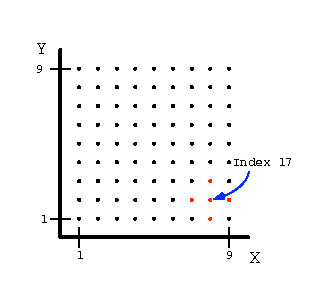
\includegraphics[scale=1.2]{figures/finite2D.eps}
  \caption{The neighboring points in two dimensions}
\label{fig:finite2D}
\end{figure}

In figure \ref{fig:finite2D} we can see that the neighboring points are no longer on a single axis. The points in red
are the points required for approximating the second derivative for point 17. Using equation \ref{eq:2ndDegreeTaylor2} as-is
will utilize points 16 and 18 but not points 8 and 26. We can accomplish this expansion by performing a tensor product
with the matrix in equation \ref{eq:kinetic2} and the identity matrix. 

The tensor product, $\otimes$, of two matrices of equal dimensions is defined as

\begin{equation}
\begin{array}{r l}
\setlength{\jot}{9pt}
\begin{bmatrix}
        A_{1,1} & A_{1,2} \\
        A_{2,1} & A_{2,2} \\
\end{bmatrix} \otimes
\begin{bmatrix}
        B_{1,1} & B_{1,2} \\
        B_{2,1} & B_{2,2} \\
\end{bmatrix} &= \begin{bmatrix}
                    A_{1,1} \begin{bmatrix}
                             B_{1,1} & B_{1,2} \\
                             B_{2,1} & B_{2,2} \\
                             \end{bmatrix} & A_{1,2} \begin{bmatrix}
                                                      B_{1,1} & B_{1,2} \\
                                                      B_{2,1} & B_{2,2} \\
                                                     \end{bmatrix} \\
 
                    A_{2,1} \begin{bmatrix}
                             B_{1,1} & B_{1,2} \\
                             B_{2,1} & B_{2,2} \\
                             \end{bmatrix} & A_{2,2} \begin{bmatrix}
                                                      B_{1,1} & B_{1,2} \\
                                                      B_{2,1} & B_{2,2} \\
                                                     \end{bmatrix} \\

                \end{bmatrix} \\
              & = \begin{bmatrix}
                    A_{1,1}B_{1,1} & A_{1,1}B_{1,2} & A_{1,2}B_{1,1} & A_{1,2}B_{1,2} \\
                    A_{1,1}B_{2,1} & A_{1,1}B_{2,2} & A_{1,2}B_{2,1} & A_{1,2}B_{2,2} \\
                    A_{2,1}B_{1,1} & A_{2,1}B_{1,2} & A_{2,2}B_{1,1} & A_{2,2}B_{1,2} \\
                    A_{2,1}B_{2,1} & A_{2,1}B_{2,2} & A_{2,2}B_{2,1} & A_{2,2}B_{2,2} \\
                   \end{bmatrix}
\end{array}
\label{eq:tensorDef}
\end{equation}

The tensor product must be performed with an identity matrix to create the proper expansion. For two dimensions
the form of the equation will be 

\begin{equation}
K = X \otimes I + I \otimes Y
\label{eq:2DTensor}
\end{equation}

Where $X$ and $Y$ represent the kinetic energy matrices for their respective dimensions and $I$ represents the 
identity matrix. Working through a small example will illustrate how this equation produces the desired results. 
The example we will use will have $N = 3$ samples per dimension, giving us a $3 \times 3$ version of the kinetic
energy matrix. This results in a two dimensional sample space of $9$ points. 

We begin by performing $X \otimes I$

\begin{equation}
\begin{bmatrix}
 -2 & 1 & 0 \\
  1 & -2 & 1 \\
  0 & 1 & -2 \\
\end{bmatrix} \otimes \begin{bmatrix}
                        1 & 0 & 0 \\
                        0 & 1 & 0 \\
                        0 & 0 & 1 \\
                      \end{bmatrix} = \begin{bmatrix}
                                        -2 & 0 & 0 & 1 & 0 & 0 & 0 & 0 & 0 \\
                                        0 & -2 & 0 & 0 & 1 & 0 & 0 & 0 & 0 \\ 
                                        0 & 0 & -2 & 0 & 0 & 1 & 0 & 0 & 0 \\
                                        1 & 0 & 0 & -2 & 0 & 0 & 1 & 0 & 0 \\
                                        0 & 1 & 0 & 0 & -2 & 0 & 0 & 1 & 0 \\
                                        0 & 0 & 1 & 0 & 0 & -2 & 0 & 0 & 1 \\
                                        0 & 0 & 0 & 1 & 0 & 0 & -2 & 0 & 0 \\
                                        0 & 0 & 0 & 0 & 1 & 0 & 0 & -2 & 0 \\
                                        0 & 0 & 0 & 0 & 0 & 1 & 0 & 0 & -2 \\
                                      \end{bmatrix}
\label{eq:tensorExample}
\end{equation}

Then perform $I \otimes Y$

\begin{equation}
\begin{bmatrix}
  1 & 0 & 0 \\
  0 & 1 & 0 \\
  0 & 0 & 1 \\
\end{bmatrix} \otimes \begin{bmatrix}
                         -2 & 1 & 0 \\
                          1 & -2 & 1 \\
                          0 & 1 & -2 \\
                      \end{bmatrix} = \begin{bmatrix}
                                        -2 & 1 & 0 & 0 & 0 & 0 & 0 & 0 & 0 \\
                                        1 & -2 & 1 & 0 & 0 & 0 & 0 & 0 & 0 \\ 
                                        0 & 1 & -2 & 0 & 0 & 0 & 0 & 0 & 0 \\
                                        0 & 0 & 0 & -2 & 1 & 0 & 0 & 0 & 0 \\
                                        0 & 0 & 0 & 1 & -2 & 1 & 0 & 0 & 0 \\
                                        0 & 0 & 0 & 0 & 1 & -2 & 0 & 0 & 0 \\
                                        0 & 0 & 0 & 0 & 0 & 0 & -2 & 1 & 0 \\
                                        0 & 0 & 0 & 0 & 0 & 0 & 1 & -2 & 1 \\
                                        0 & 0 & 0 & 0 & 0 & 0 & 0 & 1 & -2 \\
                                      \end{bmatrix}
\label{eq:tensorExample2}
\end{equation}
By adding the two resulting matrices we get
\begin{equation}
                       \begin{bmatrix}
                                        -4 & 1 & 0 & 1 & 0 & 0 & 0 & 0 & 0 \\
                                        1 & -4 & 1 & 0 & 1 & 0 & 0 & 0 & 0 \\ 
                                        0 & 1 & -4 & 0 & 0 & 1 & 0 & 0 & 0 \\
                                        1 & 0 & 0 & -4 & 1 & 0 & 1 & 0 & 0 \\
                                        0 & 1 & 0 & 1 & -4 & 1 & 0 & 1 & 0 \\
                                        0 & 0 & 1 & 0 & 1 & -4 & 0 & 0 & 1 \\
                                        0 & 0 & 0 & 1 & 0 & 0 & -4 & 1 & 0 \\
                                        0 & 0 & 0 & 0 & 1 & 0 & 1 & -4 & 1 \\
                                        0 & 0 & 0 & 0 & 0 & 1 & 0 & 1 & -4 \\
                                      \end{bmatrix}
\label{eq:finalMat}
\end{equation}

The first observation is that the diagonal is no longer $-2$ but $-4$ instead. This has to do with the relative 
amount each of the points is weighted when approximating the second derivative. In a single dimension up to two
neighbors were taken into account, for two dimensions up to four neighbors. In order to conserve the center point's
relative weight to its neighbors it is doubled here. In fact, when expanding yet again to three dimensions the 
point is tripled to $-6$. 
If we were to choose any point in our sample space we would see that the rows from the matrix result in equation 
\ref{eq:finalMat} have the appropriate coefficients. For example, if chose sample point $4$ we would expect to 
use the neighboring values, in this case points $1$, $5$ and $7$. 

\begin{figure}
\centering
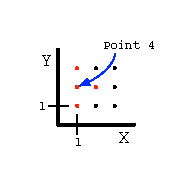
\includegraphics[scale=2.0]{figures/9PointExample.eps}
\caption{The example sample space with neighbors colored red}
\label{9PointExample}
\end{figure}

In fact, the matrix from equation \ref{eq:finalMat} has a $1$ in columns $1$, $5$ and $7$. The process from equation 
\ref{eq:2DTensor} has preserved the appropriate boundaries and expanded the system to two dimensions. Unfortunately,
it is not possible to add the third dimension as we did with the second dimension. In order to expand to three dimensions
properly the equation is

\begin{equation}
K = X \otimes I \otimes I + I \otimes Y \otimes I + I \otimes I \otimes Z
\label{eq:3DTensor}
\end{equation}

As we can see, the pattern is the same idea but extended to include a third component. When performing this expansion 
in two dimensions the two $3 \times 3$ matrices resulted in a $9 \times 9$ kinetic energy matrix. For three dimensions
this expands even further to $27 \times 27$, or $N^3 \times N^3$. This illustrates how crucial it is to utilize sparse 
matrix representations. Otherwise even relatively small sample rates will result in huge memory requirements when in fact
most of the `data' are zeros.

Creating the matrix requires two main steps. First we must set up the matrix from equation \ref{eq:kinetic2}. This is 
done using the \verb+setCoefficient+ function. The function takes two parameters, \verb+corners+ and
\verb+n+. We introduced \verb+corners+ to specify the values at the corners of the
matrix in order to experiment with different boundary conditions. The parameter \verb+n+ defines the number of samples
for each dimension. 

The function itself consists of three parts. The first section allocates an empty matrix of size $n \times n$ and 
set the diagonal and neighboring values to the appropriate coefficient. 

\begin{lstlisting}[caption={Function to create matrix of coefficients}, label=lst:setCoefficient]
    function K = setCoefficient(n, corners)
	K = zeros(n); %initialize empty matrix of size n
	
	%use determined coefficients to fill diagonal
	for i = 2:n-1
		K(i,i-1) = 1;
		K(i,i)   = -2;
		K(i,i+1) = 1;
	end
\end{lstlisting}


Note that
at this point the matrix is not a sparse matrix, this is due to the fact that full\footnote{non-sparse} matrices are
easier to manipulate in \verb+MATLAB+ than their sparse counterparts. Being $n \times n$ is still very manageable in terms
of memory resources and will be converted to a sparse matrix once any manipulation of the corners and rows has been completed. 
We perform this in the next section of the function

\begin{lstlisting}[caption={Second two parts of setting the coefficients}, label=lst:cetCoeff2, firstnumber=11]	
	%Ensure that the corners of the matrix are what we desire
	%old version that worked:
	K(1,1) = corners;
	K(1,2) = -1;
	K(n,n) = corners;
	K(n,n-1) = -1;
	
	K = sparse(K);
end	
\end{lstlisting}

Having converted the matrix to its sparse representation we now gain the memory saving benefits while having taken
advantage of the ease of manipulation when constructing the matrix. 


\section{Simulating a Quantum Dot}
Now that we have both the kinetic and potential energy matrices we can simulate the system. 


\chapter{Results and Discussion}

\chapter{Conclusion}



\section{Further Work}

\bibliography{diss}

\end{document}
